


%======================================================================
\chapter{Numerical Experiments}\label{ch3:NumExp}

\markright{PROPOSAL}
%======================================================================

\section{Simulation tools}

\paragraph{Description of what is in this chapter} Becuase yes

\subsection{LAMMPS}

\paragraph{Talk about LAMMPS} LAMMPS is a computational engine for modeling interacting particles at any length scale, so long as the interactions are primarily short-range, and particles densities are moderately bounded\citep{thompsonLAMMPSFlexibleSimulation2022}.
LAMMPS implemented MD algorithms to enable parallelism across CPUs via MPI, and some versions of these algorithms for GPUs.

For test simulations we used the mpi paralelization scheme, meanwhile the final results where computed with the serial version, since we had access to a cluster.

A LAMMPS input script (text file) is simply a series of lines each beginning with a command name followed by one or more whitespace separated arguments. 
Programming-like commands are included which define variables, perform conditional tests, execute loops, or invoke shell commands, eg to launch a program external to LAMMPS. 
The input script is parsed and executed one line at a time which means a single script can be used to run a simulation in stages, altering one or more parameters between the stages, or to run a series of independent simulations where the entire system is reinitialized multiple times.

- Pair styles
- Atom styles
- Fix styles
- Computes styles
- units definitions

\paragraph{Make a resume of } partitioning, communication, neighbr lists

Since we had access to the lavis cluster we\dots

\paragraph{Talk about the Fix styles} Fix styles implement operations performed during a dynamics timestep or an energy minimization iteration\citep{thompsonLAMMPSFlexibleSimulation2022}.
The initial\_integrate() and final\_integrate() methods of fix styles can be used to implement portions of the velocity-Verlet algorithm for various ensembles at the appropriate points in the timestep.

\paragraph{Units} Lennar Jones units.
distance $=\sigma$.
time = reduce LJ $\tau$.
mass = ratio to unitless $1.0$.
temperature = reduced LJ temp.
pressure = reduced LJ pressure
energy = $\epsilon$.
velocity = $\sigma/\tau$.
force = reduce LJ force ($\sigma/\tau^2$).
https://docs.lammps.org/99/units.html

\section{Simulation methodology}\label{ch3:SimProtocol}

\paragraph{Overview} of the simulation workflow.

The simulation methodology is based on the work presented in\citep{gnanSilicoSynthesisMicrogel2017} and\citep{sorichettiStructureElasticityModel2023}, with the objective of create a representative polymer structure of a microgel and characterize the mechanical response under shear deformation.
This methodology creates the structure by using a mixture of two types of patchy particles.
The patchy particles are spheres of identical size and mass decorated by patches to represent interaction sites.
One type represent a \textit{Crosslinker} and is define by 1 central particle with 4 patches placed at the vertices of a circumscribed tetrahedron. %in the center particle.
The other one represent a \textit{Monomer} define by 1 central particle and 2 patches placed at the poles.

\begin{comment}
\marginpar{
%Before proceeding further, it is important to mention that from now on we are going to refer to the center particle of the Crosslinker as ``CL'' and the patches as ``PA'', naturally, the center particle of the Monomer patchy particle as ``MO'' and the patches as ``PB''.
\begin{itemize}
    \item $\vec{r}_i$: Position of Crosslinker central particle
    \item $\vec{r}_j$: Position of Monomer central particle
    \item $\{\vec{r}_{\mu}^i\}$ Set of positions of the patches in the crosslinker patchy particle
    \item $\{\vec{r}_{\upsilon}^j\}$ Set of positions of the patches in the monomer patchy particle
\end{itemize}
}
\end{comment}

The interaction between the central particles is modeled with a Weeks-Chandler-Andersen repulsive potential,
\begin{gather}
    U_{WCA}(r_{i,j}) =\left\{ 
        \begin{array}{ll}
            4\epsilon_{i,j}\left[\qty(\frac{\sigma}{r_{i,j}})^{12}-\qty(\frac{\sigma}{r_{i,j}})^6\right]+\epsilon_{i,j}, & r_{i,j}\in[0,2^{1/6}\sigma], \\
            0, & r_{i,j}>2^{1/6}\sigma
        \end{array}
\right.
    ,\label{eqn:CL-MO_interaction}
\end{gather}
where $r_{i,j}$ is the distance between the center of the central particles, $\sigma$ is the diameter of the particles and $\epsilon_{i,j}$ is the energy of the interacton.
The patch-patch interaction is modeled with an attractive potential,
\begin{gather}
    U_{\mathrm{patchy}}\qty(r_{\mu\upsilon}) = \left\{
        \begin{array}{ll}
            2\epsilon_{\mu\upsilon}\left(\frac{\sigma_p^4}{2 r_{\mu\upsilon}^4}-1\right)\exp\left[\frac{\sigma_p}{\qty(r_{\mu\upsilon}-r_{c})}+2\right], & r_{\mu\upsilon}\in\qty[0,r_c], \\
            0, & r_{\mu,\upsilon}>r_c,
        \end{array}
            \right.\label{eqn:patch-patch_interaction}
\end{gather}
where $r_{\mu\upsilon}$ is the distance between two patches, $\sigma_p$ is the diameter of the patches, $r_c$ is the cut distance of interaction set to $1.5\sigma_p$ and $\epsilon_{\mu,\upsilon}$ is the interaction energy between the patches.
Moreover, the interaction between patches is complemented by a three-body repulsive potential, defined in terms of~\eqref{eqn:patch-patch_interaction}, that provides an efficient bond-swapping mechanism making possible to easily equilibrate the system at extremely low temperatures, while at the same time, reataining the single-bond-per-patch condition\citep{sciortinoThreebodyPotentialSimulating2017},
\begin{gather}
    U_{\mathrm{swap}}(r_{l,m},r_{l,n}) = w\sum_{l,m,n}\epsilon_{m,n}U_3\qty(r_{l,m})U_3\qty(r_{l,n}),\quad r_{l,n}\in\qty[0,r_c],\label{eqn:swap_interaction}
\end{gather}
where
\begin{gather}
    U_{3}\qty(r) = \left\{
        \begin{array}{ll}
            1 & r\in\qty[0,r_{\min}], \\
            -U_{\mathrm{patchy}}\qty(r)/\epsilon_{m,n}, & r\in\qty[r_{\min},r_c]
        \end{array}
        \right.\label{eqn:swapmod_interaction}.
\end{gather}
The sum in~\eqref{eqn:swap_interaction} runs over all triples of bonded patches (patch $l$ bonded both with $m$ and $n$).
$r_{l,m}$ and $r_{l,n}$ are the distances between the reference patch and the other two patches.
The parameter $\epsilon_{m,n}$ is the energy of repulsion and $w$ is used to tuned the swapping ($w=1$) and non-swapping bonds ($w\gg1$). 
The cut off distance $r_c$ is the same as in the potential of interaction between patches, meanwhile the minimum distance $r_{\min}$ is the distance at the minimum of~\eqref{eqn:patch-patch_interaction}, \textit{i.e.} $\epsilon_{m,n}\equiv\abs{U_{\mathrm{patchy}}(r_{\min})}$.
Finally, the energy of interaction between crosslinker patches ($\epsilon_{\mu^i,\mu^i}$) are set to $0$ to allow only crosslinker-monomer and monomer-monomer bonding (figure~\ref{fig:intento2}).

\begin{figure}[ht]
    \centering 
    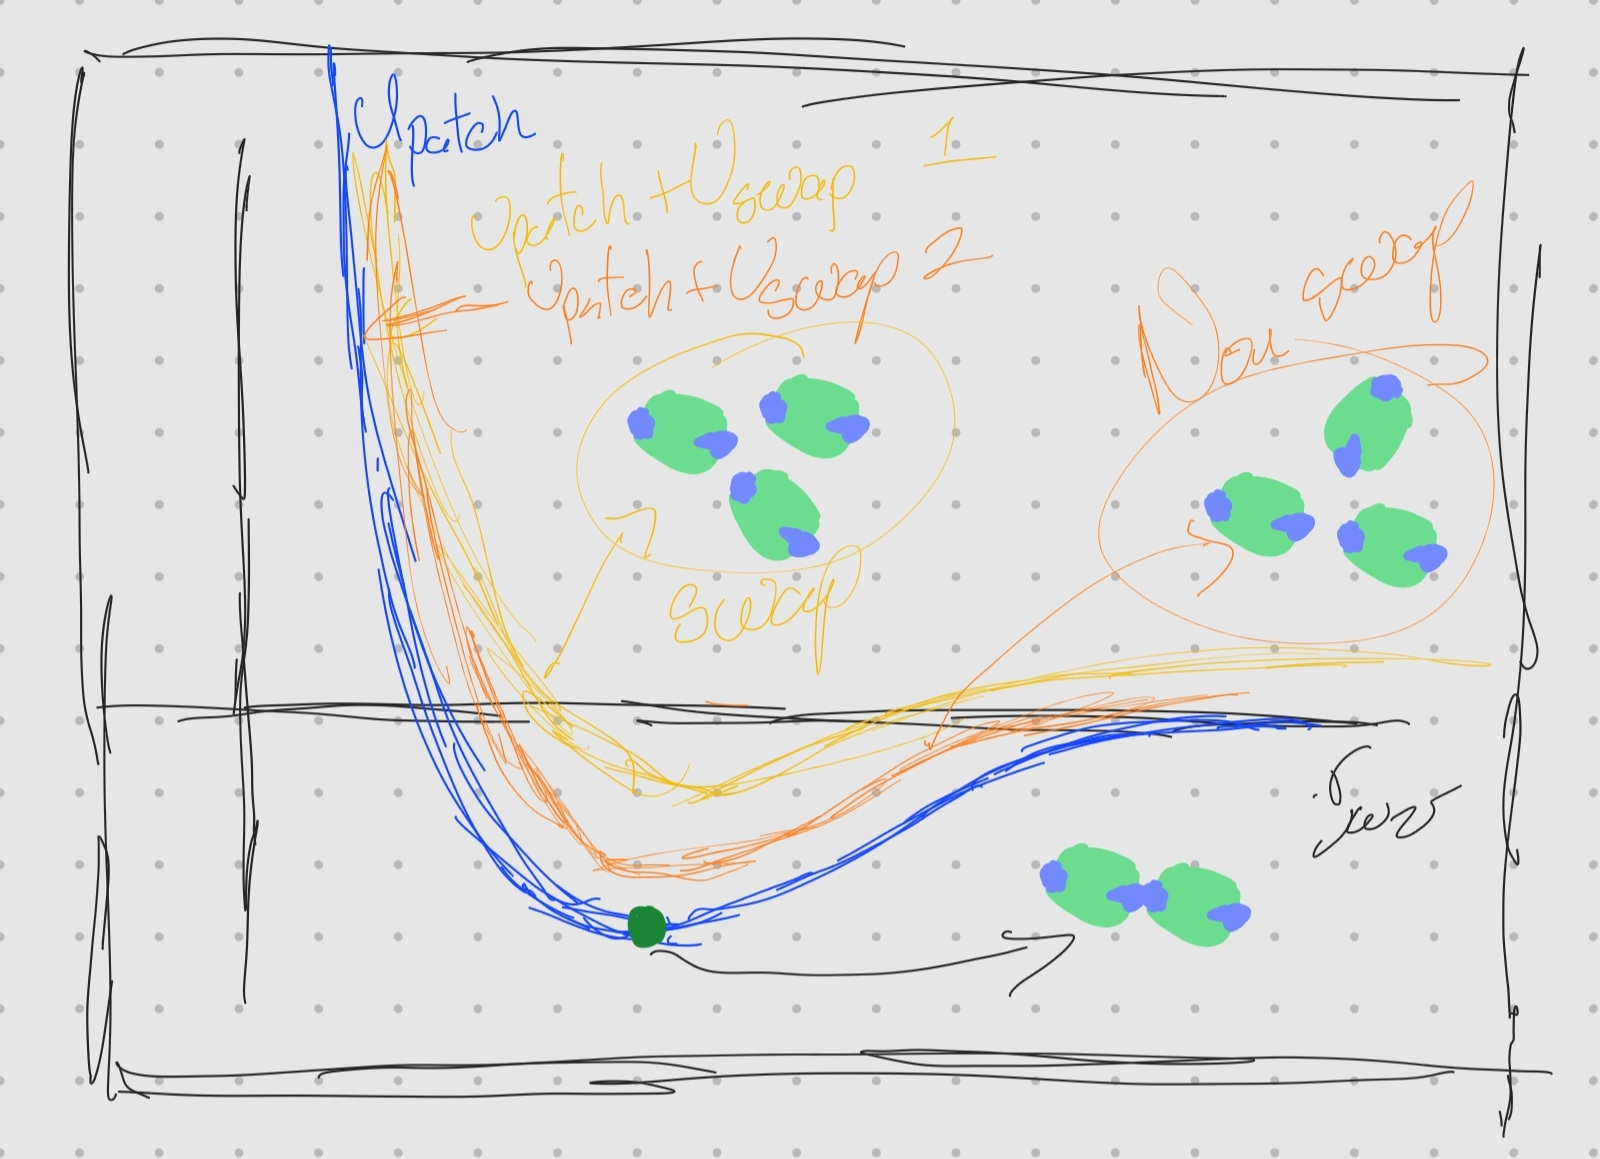
\includegraphics[width=0.8\textwidth]{figs/potentia-interactions.jpg}
    \caption{La idea de la figura es poner el pontecial de interacción entre paches y ver el efecto del pontecial de 3 cuerpos cuando $w=1$ y cuando $w\gg1$.}\label{fig:intento}
\end{figure}


\begin{figure}[ht]
    \centering 
    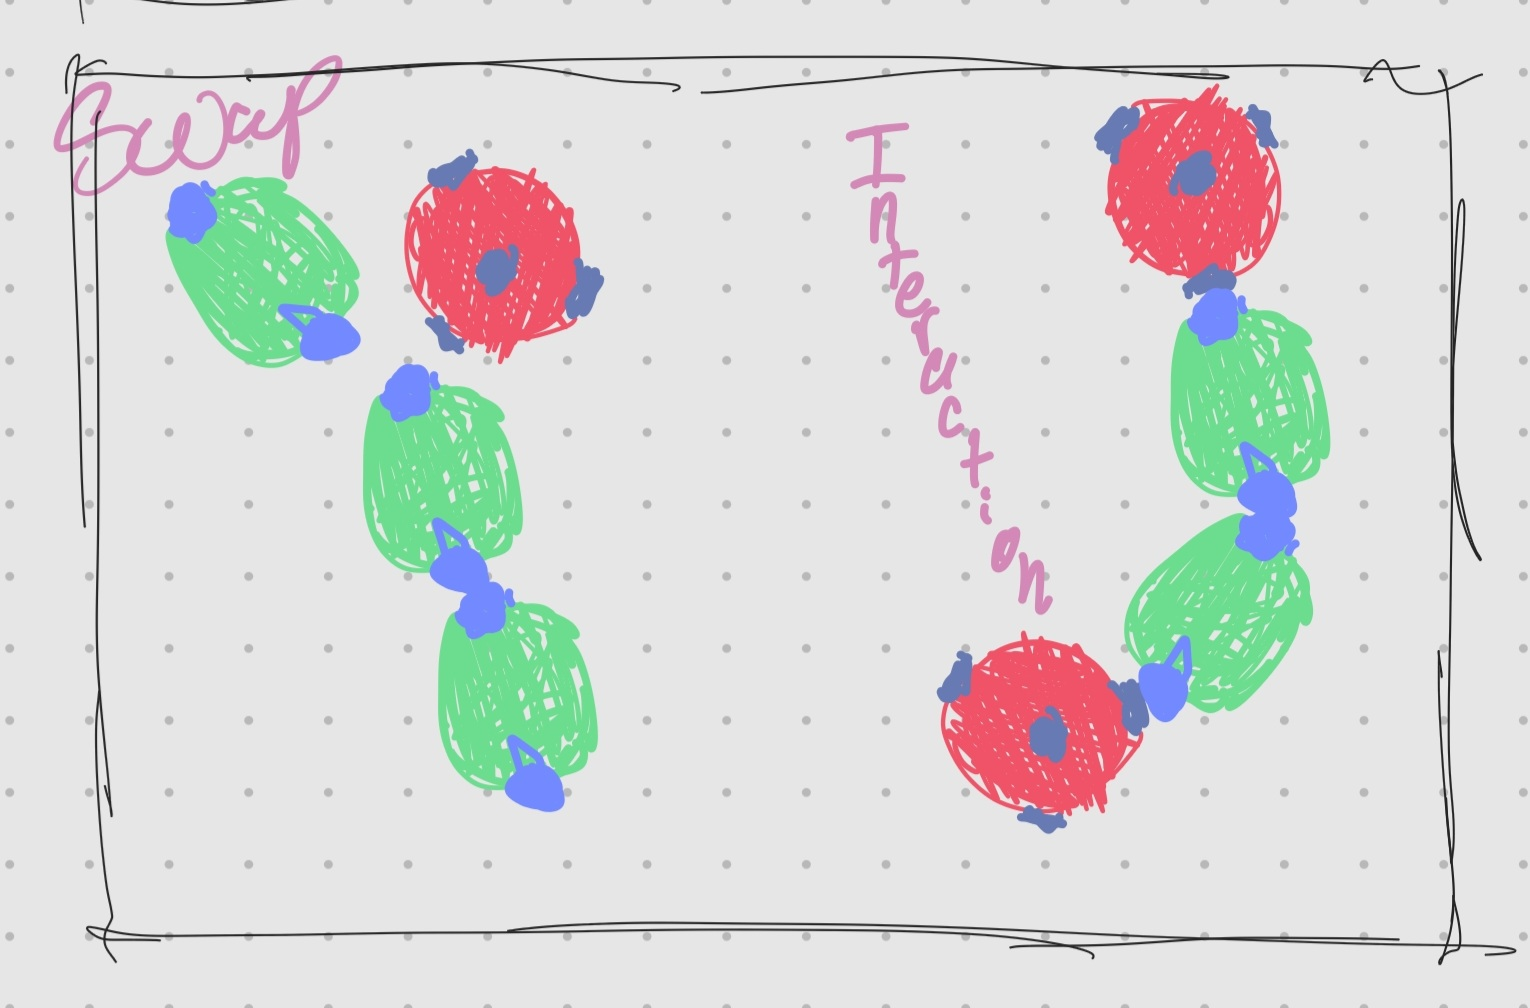
\includegraphics[width=0.8\textwidth]{figs/patches-interaction.jpg}
    \caption{La idea de esta es mostrar las posibles configuraciones (monomero-monomero, monomero-crosslinker y un poco de pontecial de 3 cuerpos)}\label{fig:intento2}
\end{figure}

\subsection{Assembly protocol}

We perform molecular dynamics (MD) simulations at fixed temperature $T = kBT/\epsilon = 0.05$, where kB is the Boltzmann constant. 
Thanks to such a low temperature, the system tends to maximize the number of bonds. 
In addition, owing to the bondswapping mechanism, the system is able to continuously restructure itself, until the large majority of possible bonds are formed.
It is important to said that the main difference between the articles cited and the implementation in this htesis are the absence of FENE bonds and the swelling potential.

\subsection{Shear protocol}

\paragraph{Parameters discussion} because yes, why shear rate and that stuff and discussion obout the damp

\paragraph{Figures} about the deformation?

\section{Results}\label{ch3:Results}

\subsection{Network analysis}

\paragraph{After} the shear

\paragraph{Before} the shear

\subsection{Mechanical response}

\paragraph{Varying shear rates and stuff}

\newpage
